\documentclass{article}

\title{Lab 3 - Mouse callback and color segmentation\\
	\large{Computer Vision}}
\author{Alberto Pasqualetto, 2121718}
\date{7 April 2024}

\usepackage[english]{babel}
% \usepackage{parskip}
\usepackage{float}
\usepackage{graphicx}
\usepackage{caption}
\usepackage{subcaption}
\graphicspath{ {./img/} }
\usepackage{cleveref}
\usepackage{xcolor}
\definecolor{redrecolor}{RGB}{201,37,92}


% \newcommand{\mV}{\,\mathrm{mV}}


\begin{document}
\maketitle


\section*{Task 1}
In task 1 an image is required to be loaded and displayed; the reference image is shown in figure \ref{fig:original}.
\begin{figure}[H]
	\centering
	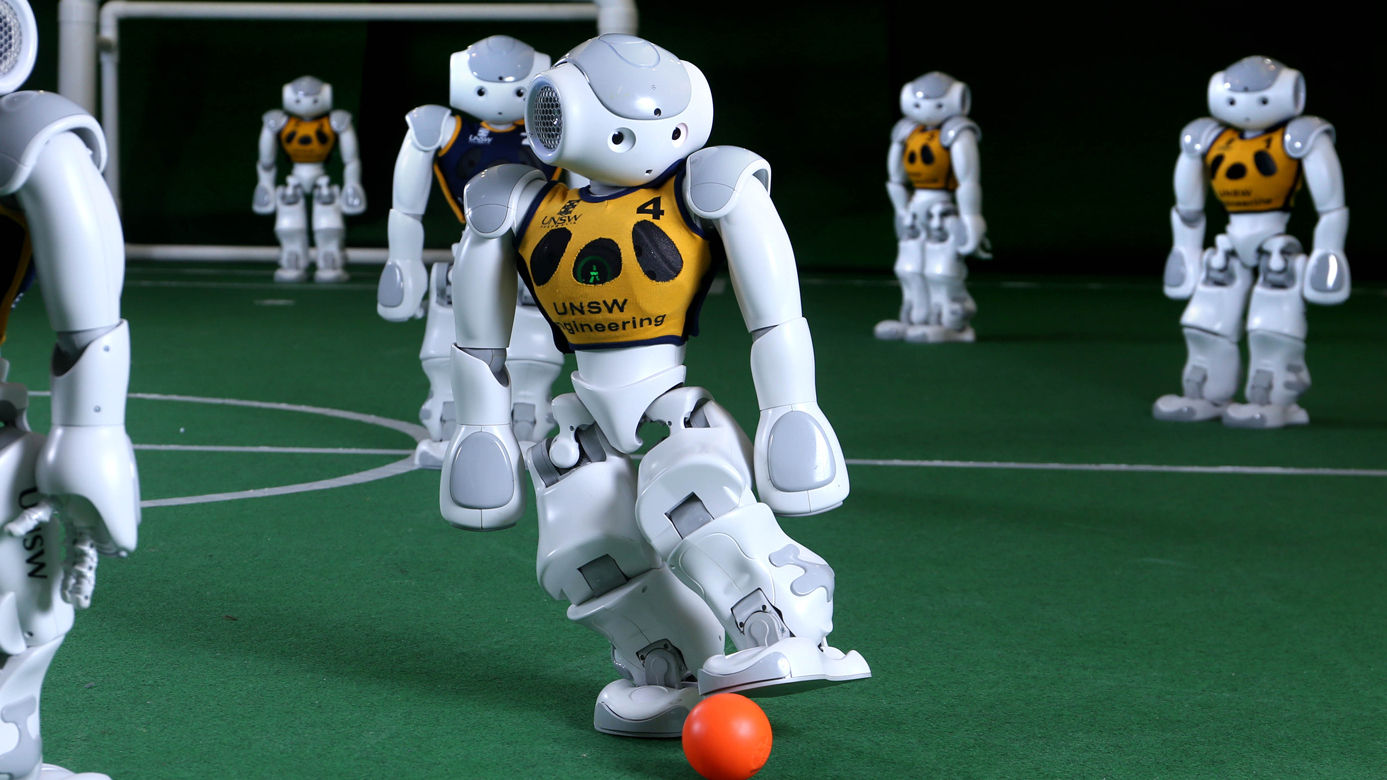
\includegraphics[width=0.8\textwidth]{../robocup.jpg}
	\caption{Original image}
	\label{fig:original}
\end{figure}


\section*{Task 2}
Task 2 requires to write a callback function which is triggered when the user clicks on the image. The callback function should print the BGR values of the pixel in that position.
A callback function is attached to a specific window using the function \texttt{cv::setMouseCallback(winname, callbackfunction)}.

The callback function is of type \texttt{cv::MouseCallback}, and it needs parameters \texttt{event}, \texttt{x}, \texttt{y}, \texttt{flags}, and \texttt{userdata}.
\texttt{event} is the event that triggered the callback: in our case we need to check if the event is a left click (\texttt{cv::EVENT\_LBUTTONDOWN}).
\texttt{userdata} is a pointer of type \texttt{void} which can be used to pass additional data to the callback function. In our case we pass the image to the callback function, so that we can access the pixel values.
\texttt{x} and \texttt{y} are the coordinates of the pixel clicked by the user which will be used to access the pixel values in the image.


\section*{Task 3}
Task 3 asks to calculate the mean of the BGR values of the pixels in the 9x9 neighborhood of the clicked pixel; the mean is calculated for each channel separately.

This code must be implemented in a callback function, expanding the one written for task 2.


\section*{Task 4}
Task 4 requires to implement a color segmentation algorithm which creates a mask of the image where only the pixels with a color similar to the one clicked by the user are shown as white pixels (255 value for a \texttt{uchar} type), the others are set to black, so we can start from a \texttt{Mat::zeros} and only color the white pixels.

Similarity is defined by a threshold (\texttt{T}) on the Euclidean distance between the BGR values of the pixel (for all pixels) and the mean BGR values in the 9x9 neighborhood of the clicked pixel from task 3.

Some results are shown in figure \ref{fig:maskBGR}: masks change depending on the clicked pixel even if the click is performed on the same object since it can have (slightly) different color values as shown in figures \labelcref{fig:maskBGR100upshirt,fig:maskBGR100downshirt}; masks obviously change by clicking on different objects in the image as shown in figures \labelcref{fig:maskBGR100robot,fig:maskBGR100floor} and when the threshold is changed as shown in figures \labelcref{fig:maskBGR25shirt,fig:maskBGR250shirt}.
\begin{figure}[H]
	\centering
	\begin{subfigure}{0.4\textwidth}
		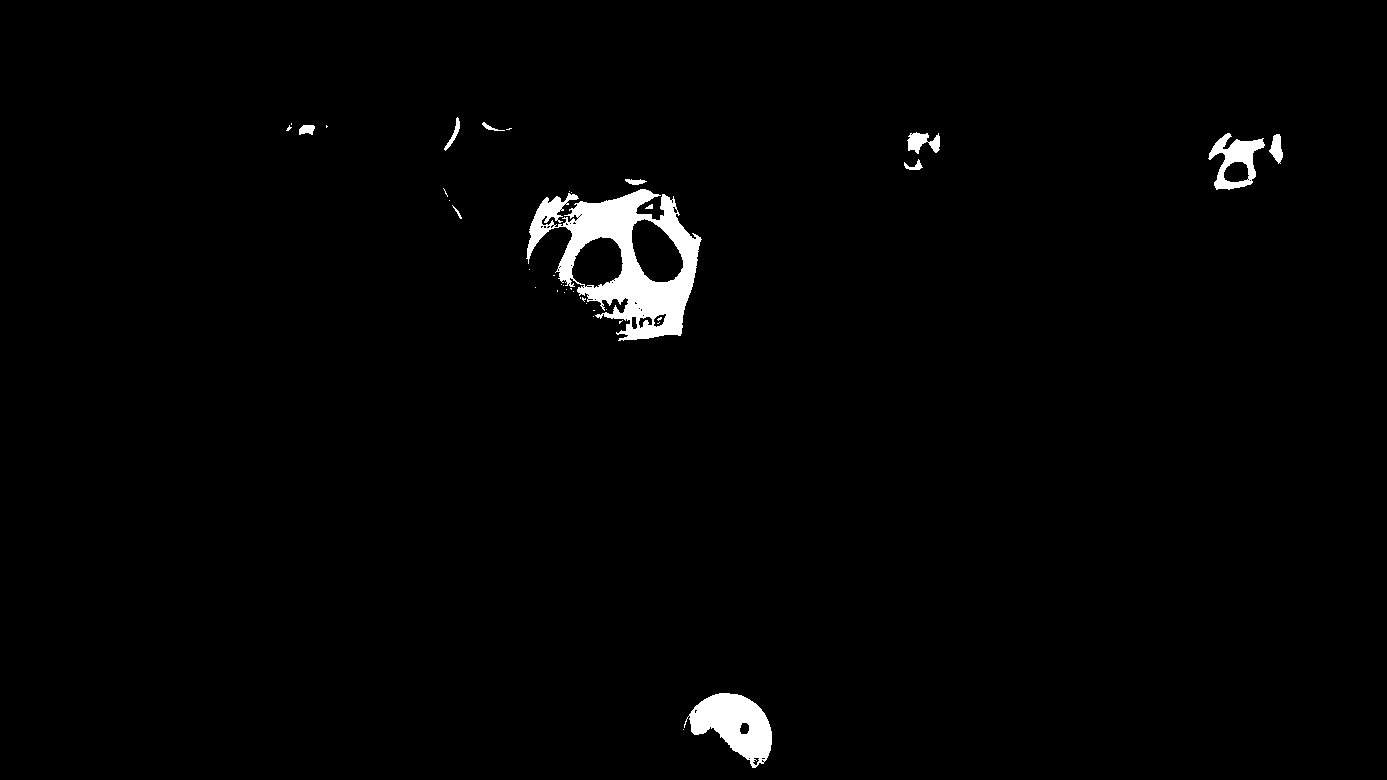
\includegraphics[width=\textwidth]{robocup_maskBGR100upshirt.jpg}
		\caption{Mask created from the upper part of the t-shirt of the robot in the foreground, threshold 100}
		\label{fig:maskBGR100upshirt}
	\end{subfigure}
	\hfill
	\begin{subfigure}{0.4\textwidth}
		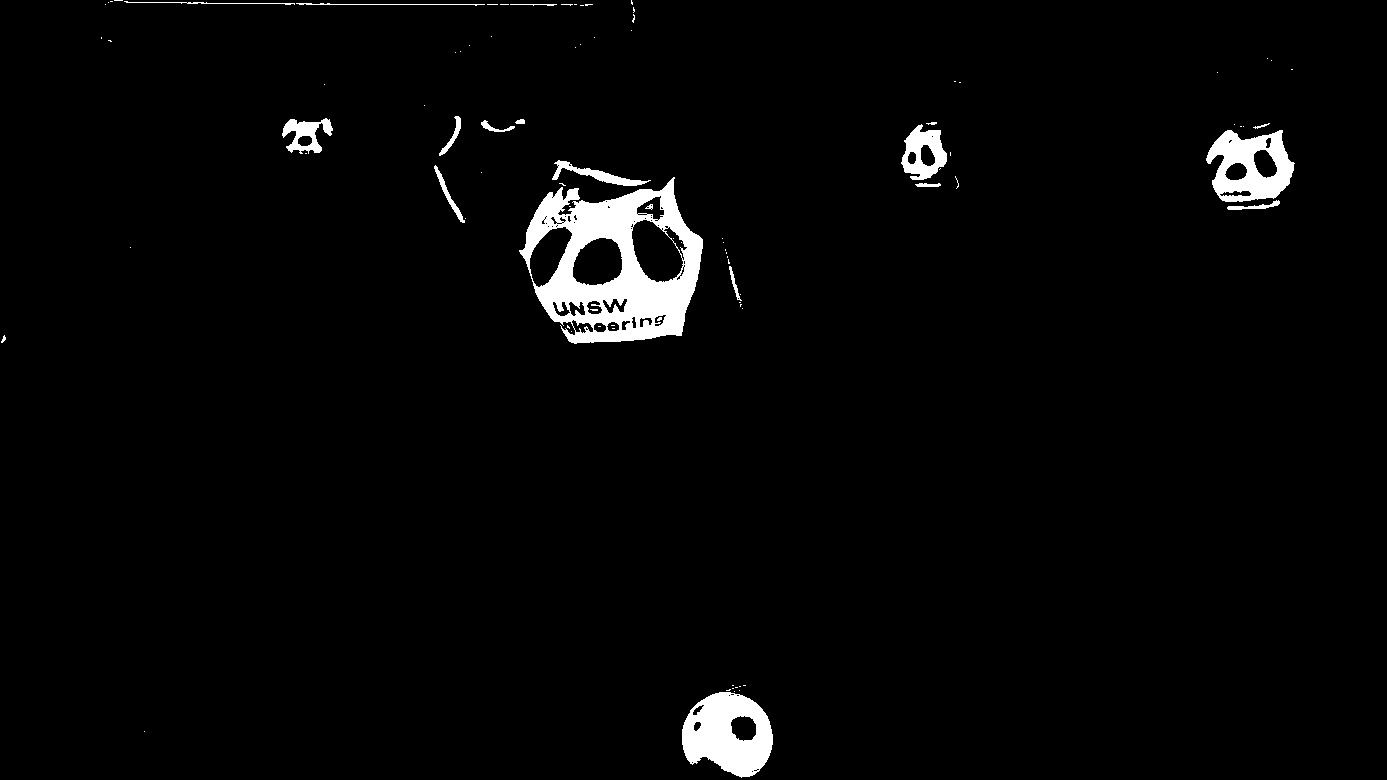
\includegraphics[width=\textwidth]{robocup_maskBGR100downshirt.jpg}
		\caption{Mask created from the lower part of the t-shirt of the robot in the foreground, threshold 100}
		\label{fig:maskBGR100downshirt}
	\end{subfigure}

	\begin{subfigure}{0.4\textwidth}
		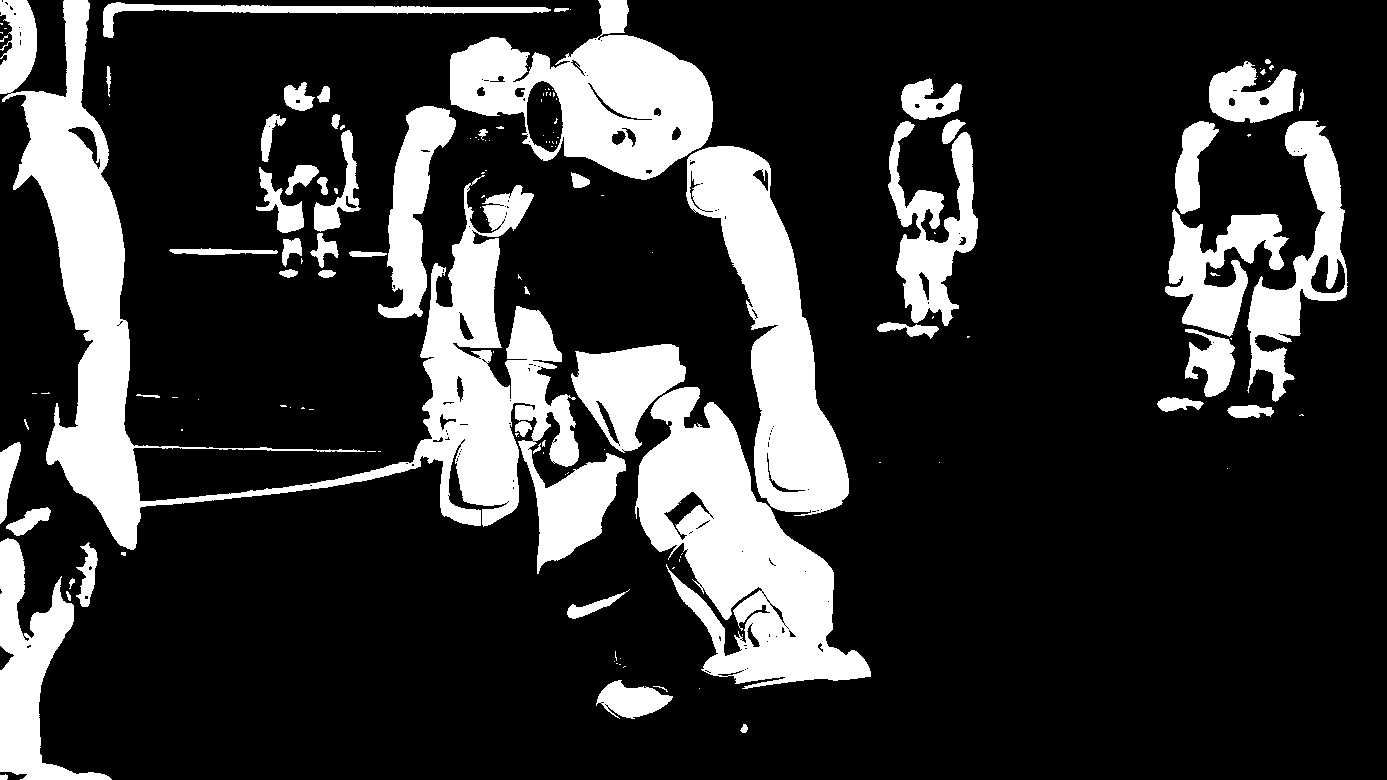
\includegraphics[width=\textwidth]{robocup_maskBGR100robot.jpg}
		\caption{Mask created from the robot body in the foreground, threshold 100}
		\label{fig:maskBGR100robot}
	\end{subfigure}
	\hfill
	\begin{subfigure}{0.4\textwidth}
		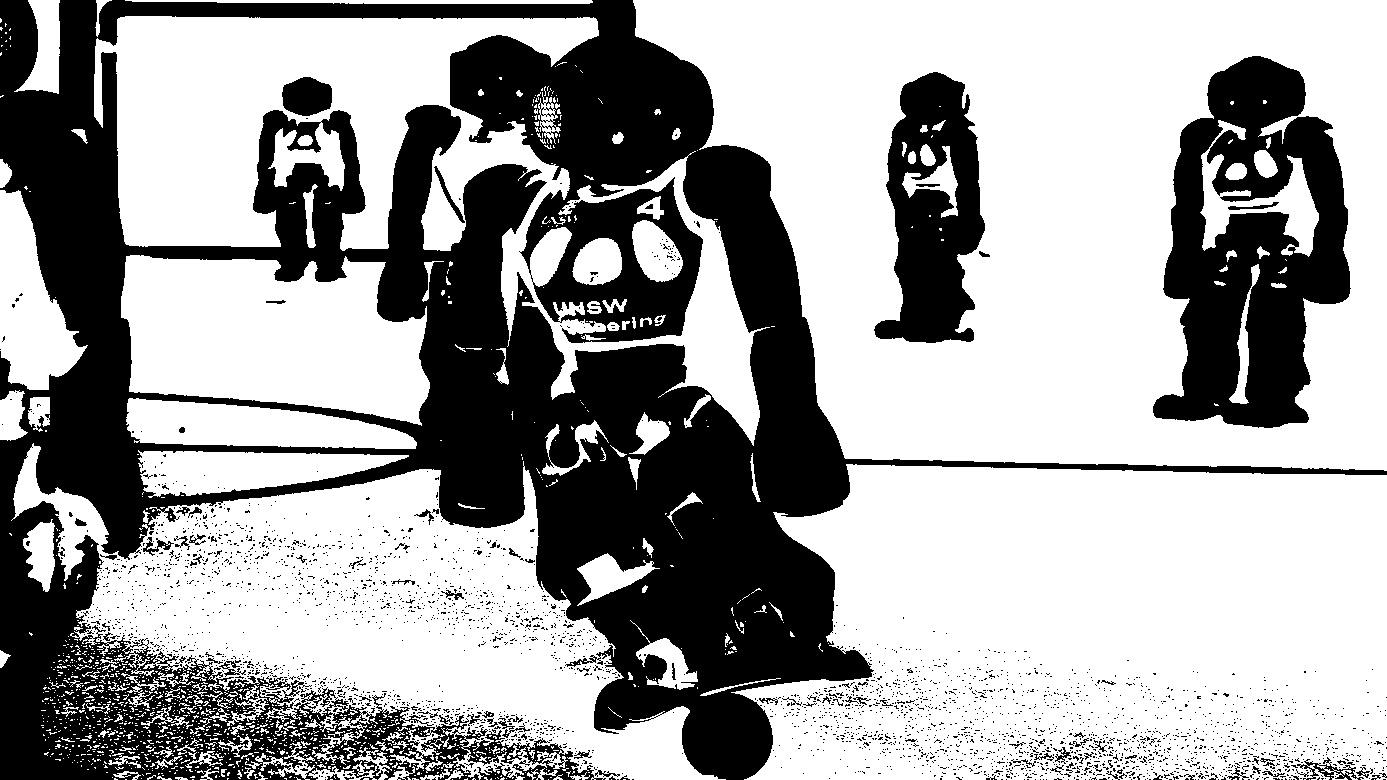
\includegraphics[width=\textwidth]{robocup_maskBGR100floor.jpg}
		\caption{Mask created from the floor, threshold 100}
		\label{fig:maskBGR100floor}
	\end{subfigure}

	\begin{subfigure}{0.4\textwidth}
		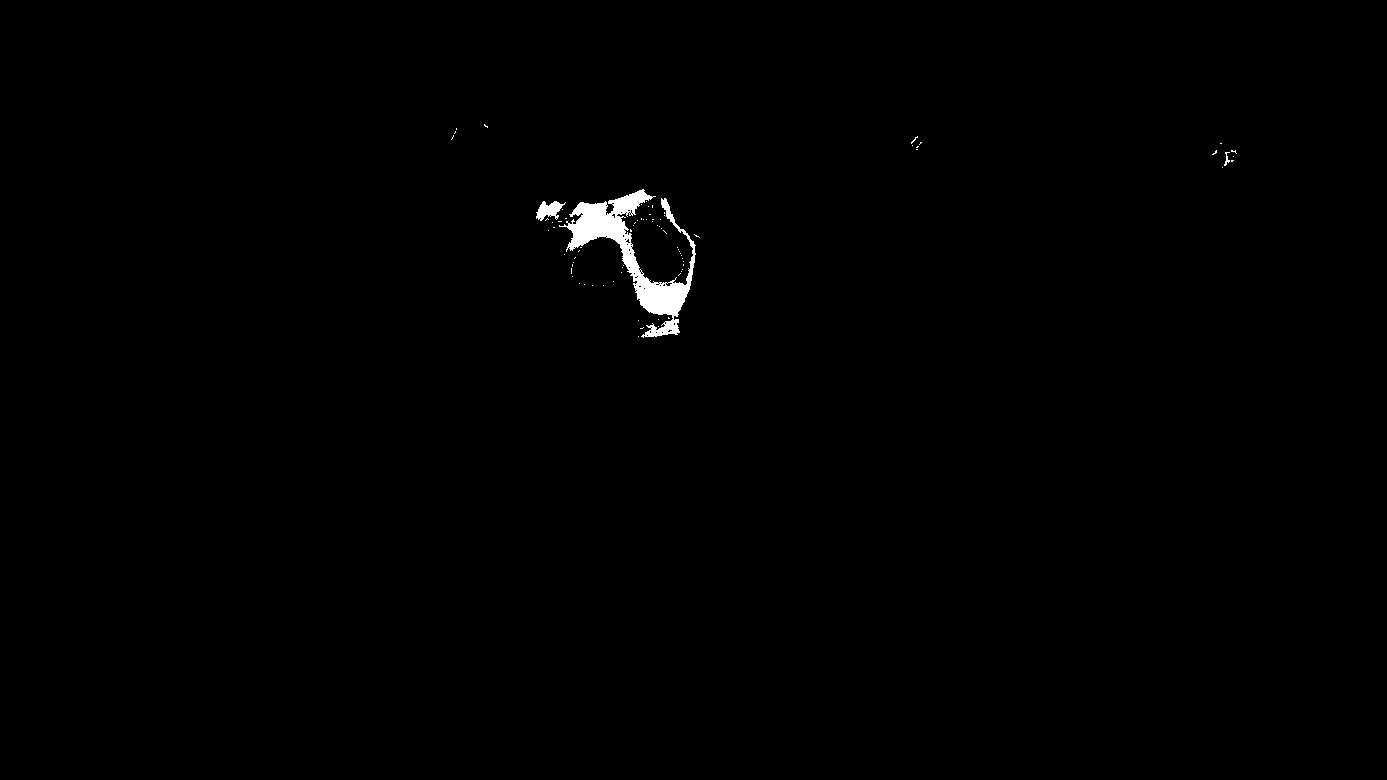
\includegraphics[width=\textwidth]{robocup_maskBGR25shirt.jpg}
		\caption{Mask created from the t-shirt of the robot in the foreground, threshold 25}
		\label{fig:maskBGR25shirt}
	\end{subfigure}
	\hfill
	\begin{subfigure}{0.4\textwidth}
		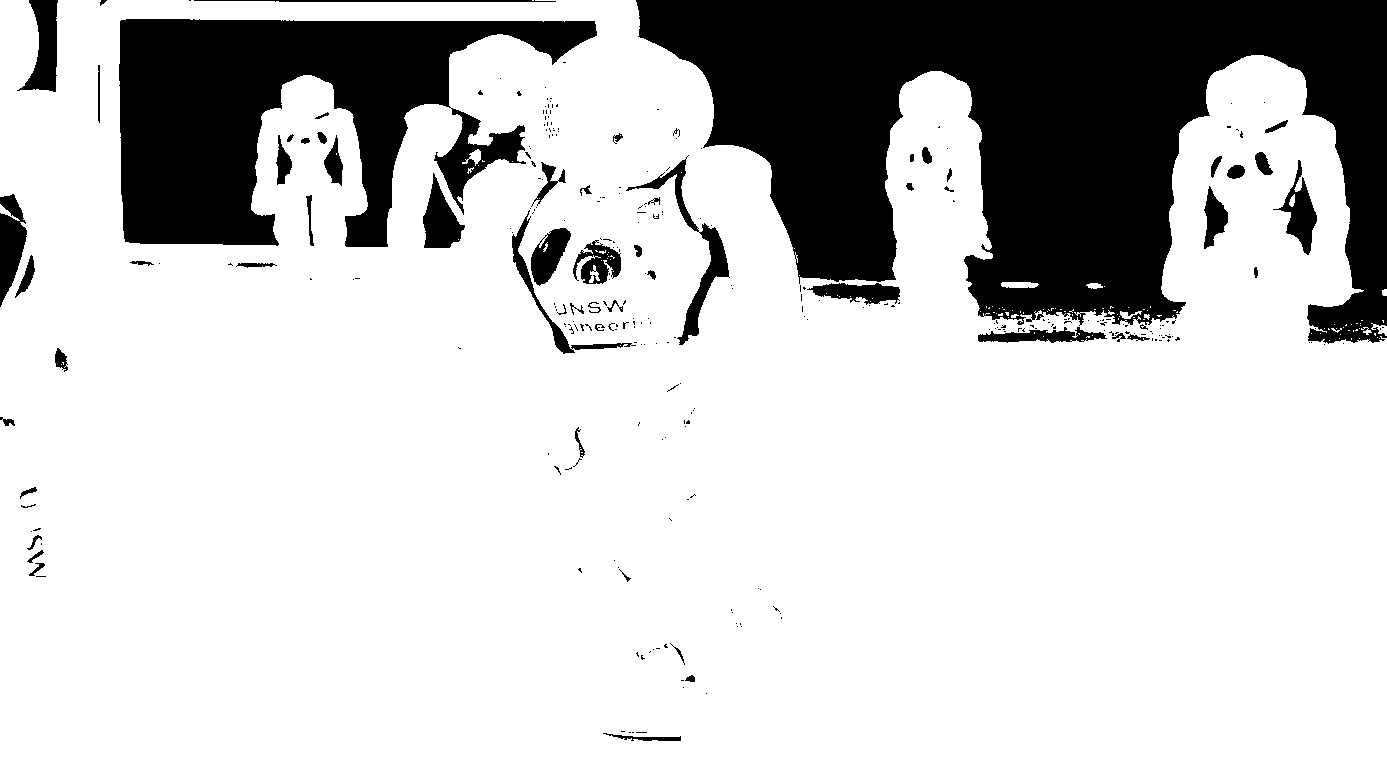
\includegraphics[width=\textwidth]{robocup_maskBGR250shirt.jpg}
		\caption{Mask created from the t-shirt of the robot in the foreground, threshold 250}
		\label{fig:maskBGR250shirt}
	\end{subfigure}
	\caption{Masks}
	\label{fig:maskBGR}
\end{figure}


\section*{Task 5}
In task 5 the same operation as in task 4 is performed, but the mask is created using the HSV color space instead of the BGR color space. The HSV color space is used because it is more intuitive to define a color range in the HSV color space than in the BGR color space.

Changing the color space (using the function \texttt{cv::cvtColor(src, dst, cv::COLOR\_BGR2HSV)}) the results are usually better and sharper, as shown in figure \ref{fig:maskHSVeuclideandist}.
\begin{figure}[H]
	\centering
	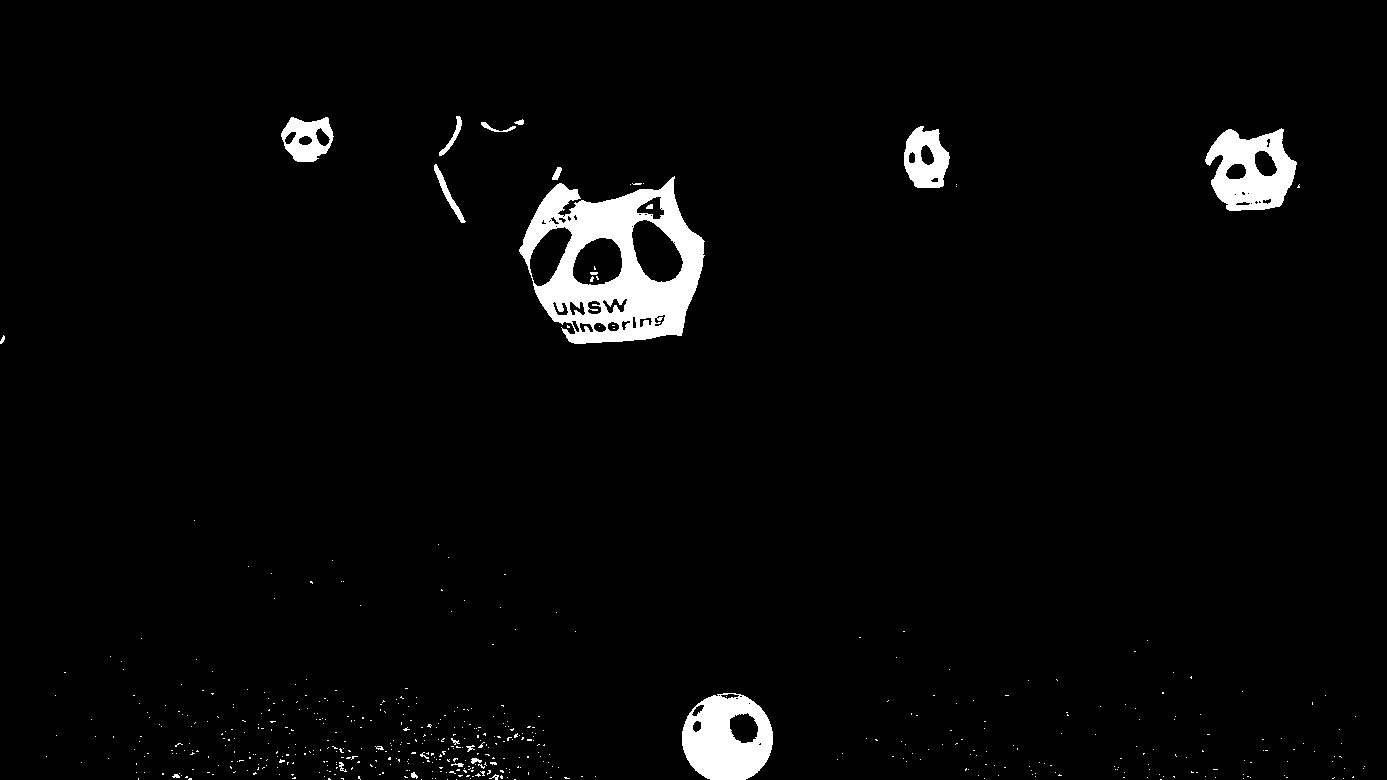
\includegraphics[width=0.8\textwidth]{robocup_maskHSVeuclideandist100shirt.jpg}
	\caption{Mask created from the t-shirt of the robot in the foreground, threshold 100, using the HSV color space and Euclidean distance}
	\label{fig:maskHSVeuclideandist}
\end{figure}

In order to exploit the HSV color space, the distance can also be calculated using only the hue channel, since we want to isolate a limited color range, giving us better result: a better segmentation can be seen in figure \ref{fig:maskHSVhuedist} (false positives can be removed afterwards since they are outliers).
\begin{figure}[H]
	\centering
	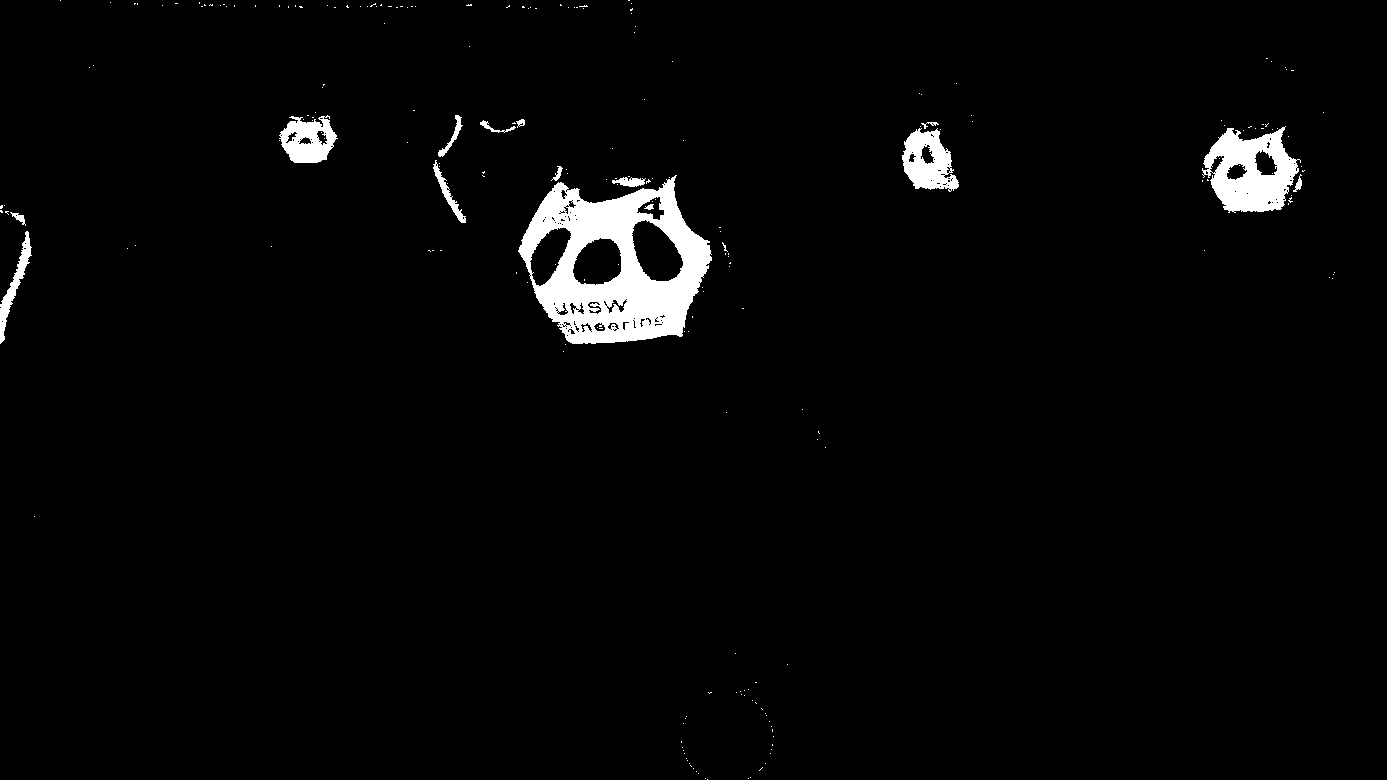
\includegraphics[width=0.8\textwidth]{robocup_maskHSVhuedist5shirt.jpg}
	\caption{Mask created from the t-shirt of the robot in the foreground, threshold 5, using the HSV color space and hue distance}
	\label{fig:maskHSVhuedist}
\end{figure}


\section*{Task 6}
In task 6 it is required to implement the color segmentation from task 4 (using BGR color space) and apply the mask to the original image recoloring the pixels in the mask with a different color: BGR(92, 37, 201) \fcolorbox{black}{redrecolor}{\rule{0pt}{3pt}\rule{3pt}{0pt}} . The result is shown in figure \ref{fig:recolorBGRbad}.

\begin{figure}[H]
	\centering
	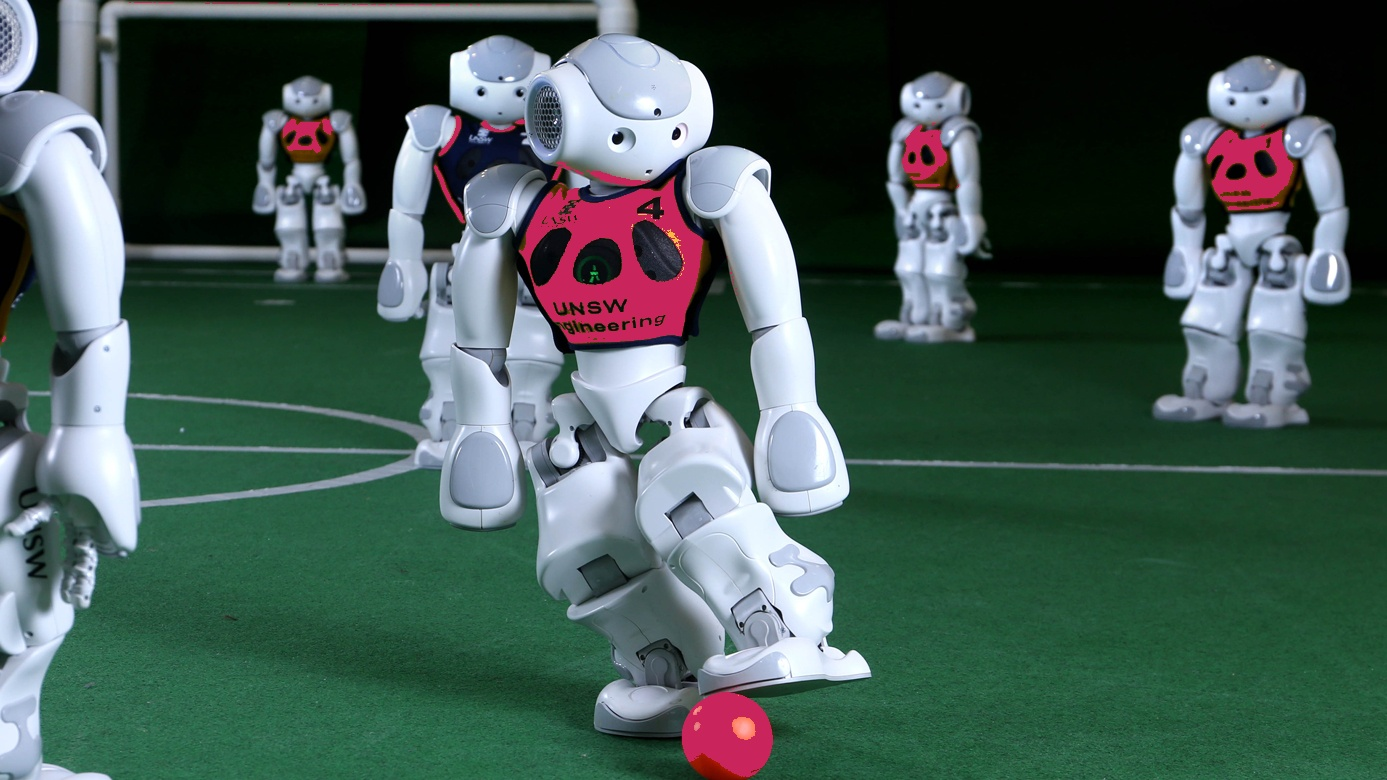
\includegraphics[width=0.8\textwidth]{robocup_recolorBGR100shirt.jpg}
	\caption{Recolored image using the mask created from the t-shirt of the robot in the foreground, threshold 100}
	\label{fig:recolorBGRbad}
\end{figure}

Distinguishing pretty similar colors like the yellow of the t-shirts and the orange of the ball is very hard using the BGR color space, as shown in figure \ref{fig:recolorBGRbad} where the ball is also recolored.

Overall, adjusting the thresholds, the results can be pretty good as shown in figure \ref{fig:recolorBGRbetter}.
\begin{figure}[H]
	\centering
	\begin{subfigure}{0.4\textwidth}
		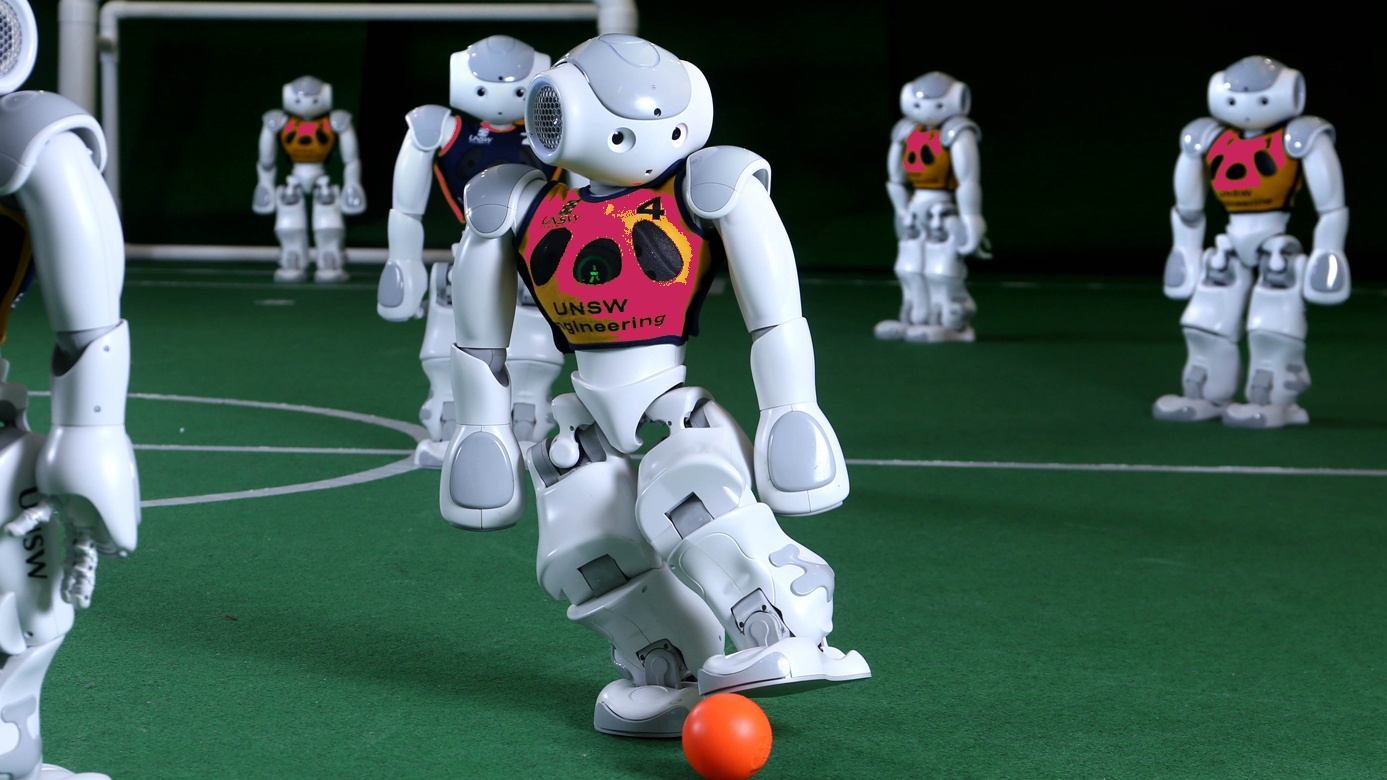
\includegraphics[width=\textwidth]{robocup_recolorBGR60shirt.jpg}
		\caption{Recolored image using the mask created from the t-shirt of the robot in the foreground, threshold 60}
	\end{subfigure}
	\hfill
	\begin{subfigure}{0.4\textwidth}
		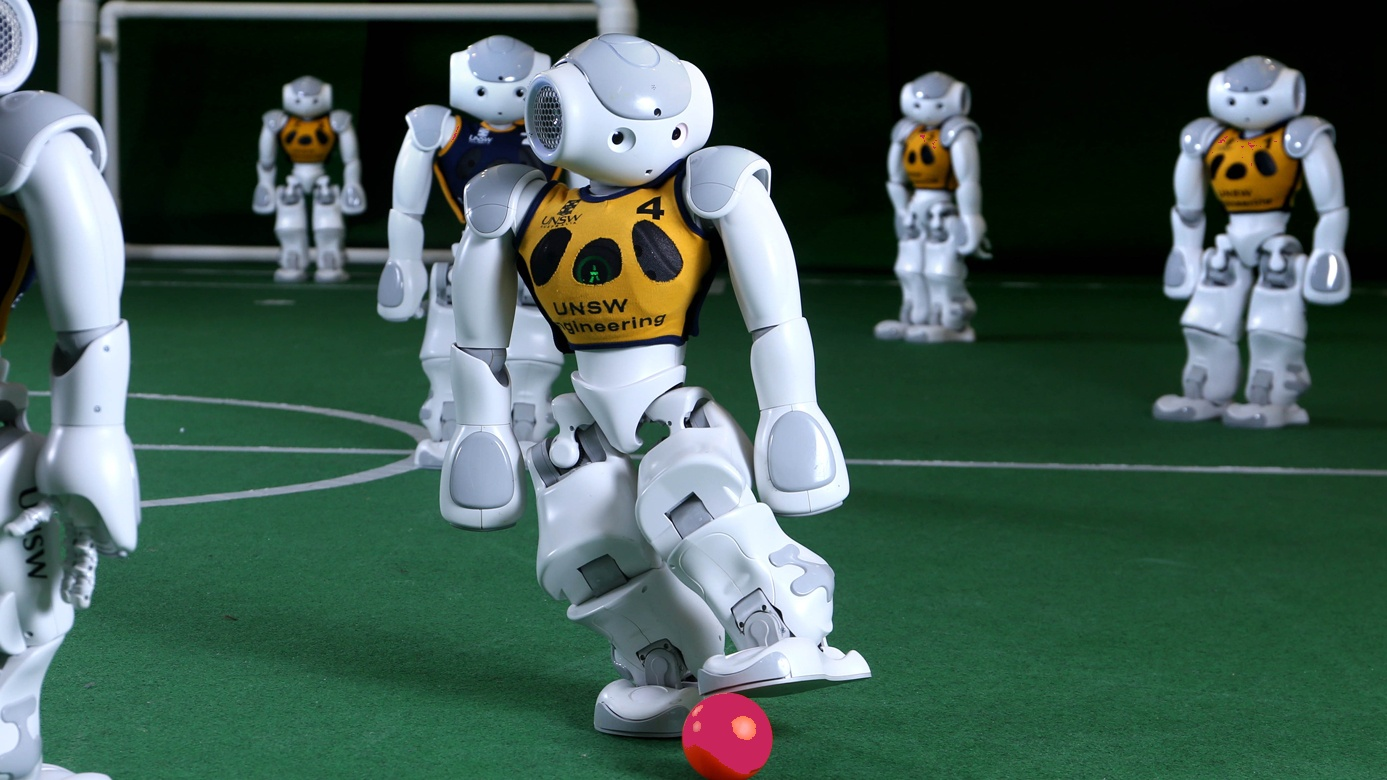
\includegraphics[width=\textwidth]{robocup_recolorBGR75ball.jpg}
		\caption{Recolored image using the mask created from the ball, threshold 75}
	\end{subfigure}
	\caption{Recolored images with adjusted thresholds}
	\label{fig:recolorBGRbetter}
\end{figure}


\end{document}
